\chapter{}
Wiederholung was ist eine Basis einer Topologie?
\dfn{Basis einer Topologie}
{
    Sei $(X, \mathcal{T})$ ein topologischer Raum. Eine Menge 
    $\mathcal{B} \subseteq \mathcal{T}$ heißt \textbf{Basis} der Topologie 
    $\mathcal{T}$, wenn für jedes $O \in \mathcal{T}$ eine Teilmenge 
    $\mathcal{B}_O \subseteq \mathcal{B}$ existiert, so dass
    $$
        O = \bigcup_{B \in \mathcal{B}_O} B .
    $$
}
Die Frage konnte sich mein imaginärer Läser jetzt sehr schnell durch 
weiterlesen beantworten.\\
Ein andere Frage die ich mir stelle ist:\\
Die Vorlesungsprüfung umfasst den Stoff der Vorlesung jedoch zb, 
der Begriff der Basis wurde in der Übung eingeführt.
Wäre die Basis nicht wiederholt worden, wäre sie dann prüfungsrelevant?



Aber naje $\dots$ Weiter mit Stoff:
Zur einleitung ein äher Kreifbares Beispiel.

\ex{}
{Sei $(X, \mathcal{T})$ ein Metrischer Raum.
Und $\mathcal{T}_d$ die von der Metrik induzierte Topologie.
Dann ist $$
\mathcal{B} = \{ U_{\frac{1}{n}}(x) : x \in X, n \in \mathbb{N} \}
$$
eine Basis der Topologie $\mathcal{T}_d$.
}

\dfn{Subbasis}
{
    Sei $(X, \mathcal{T})$ ein topologischer Raum. Eine Menge 
    $\mathcal{S} \subseteq \mathcal{P}(X)$ heißt \textbf{Subbasis} 
    der Topologie 
    $$
    : \Leftrightarrow \mathcal{T}
    \text{ ist die kleineste Topologie,
     die } \mathcal{S} \text{ umfasst. }
    $$
}

\begin{figure}[h!]
 \centering
    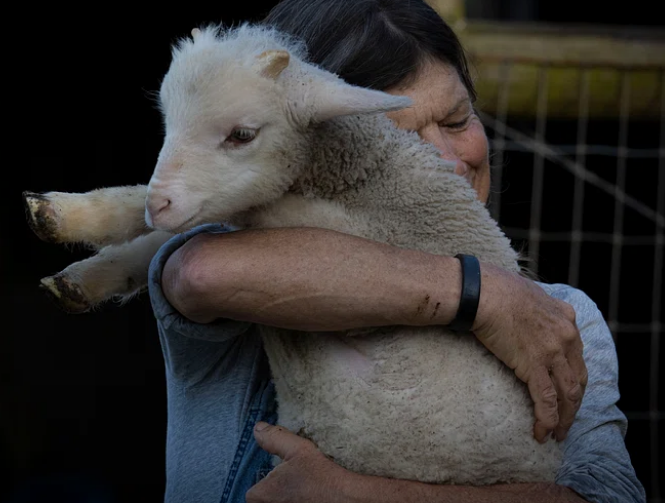
\includegraphics[width=0.6\textwidth]{pictures/hug_lemma.png}
    \caption{\url{https://creativecommons.org/licenses/by-nd/4.0/}\\
    Mensch Umfasst Lamm (Lemmachen).\\
    Wäre der Mensch die kleinste Topologie, 
    die das Lamm umfasst,\\
    so wäre der Mensch eine Subbasis.$\dots$ missed chance}
 \end{figure}


 \ex{}
 {
Sei $X \neq \emptyset \mathcal{T}_x, x \in X$  ein topologischer Raum 
 auf $\mathcal{T_x}$.
 Die Produkttopologie auf $ \prod_{x \in X} \mathcal{T}_1$ auf 
 $\prod_{x \in X} \mathcal{T}$
 $$
 S:= \{ \pi_x^{-1}(O_x) : x \in X, O_x \subseteq \mathcal{T}_x \}
 $$
    ist eine Subbasis für $\prod_{x \in X} \mathcal{T}_x$.
 }

\thm{}
{
    $\langle X, \mathcal{T} \rangle$ ein topologischer Raum und 
    $K \subseteq X$. Dann sind folgende Aussagen äquivalent:
    \begin{itemize}
        \item[(i)] $X$ ist kompakt. 
        ($\forall C \subseteq \mathcal{T}), 
        \cup C = X \Rightarrow \exists \tilde{C} 
        \subseteq C$ endlich mit $\cup \tilde{C} = X$)
        \item[(i*)] Sei $\mathcal{B}$ eine Basis von $\mathcal{T}$.
        Dann gilt:
        $$
        \forall C \subseteq \mathcal{B}, 
        \cup C = X \Rightarrow \exists \tilde{C} 
        \subseteq C \text{ endlich mit } \cup \tilde{C} = X .
        $$
        \item[(i**)] Sei $(A_i)_{i \in I}$ eine Familie abgeschlossener 
        Mengen in 
        $X$, für die gilt:
        $$
        (\forall \text{ endliches } J \subseteq I :
        \bigcap_{j \in J} A_j \neq \emptyset) \Rightarrow
        \bigcap_{i \in I} A_i \neq \emptyset .
        $$
        \item[(ii)] Sei $\mathcal{S}$ eine Subbasis von $\mathcal{T}$.
        Dann gilt:
        $$
        \forall C \subseteq \mathcal{S}, 
        \cup C = X \Rightarrow \exists \tilde{C} 
        \subseteq C \text{ endlich mit } \cup \tilde{C} = X .
        $$  
        \item[(iii)] Jedes Netz in $X$ hat ein Teilnetz,
         welches einen Grenzwert hat
    \end{itemize}
}

\begin{proof}
    \begin{itemize}
        \item{[(i) $\Rightarrow$ (i*)]}:
        Klar, da jede Basis eine Teilmenge der Topologie ist.
        \item{[(i*) $\Rightarrow$ (i)]}: 
        Sei $C \subseteq \mathcal{T}$ mit $\cup C \supseteq K$ beliebig.\\
        Für jedes $O \in C$ gibt es eine Teilmenge 
        $\mathcal{B}_O \subseteq \mathcal{B}$ mit
        $$
            O = \bigcup_{B \in \mathcal{B}_O} B .
        $$
        Also gilt: 
        $$
        \cup C = \bigcup_{O \in C} O 
        = \bigcup_{O \in C} \bigcup \mathcal{B}_O
        $$
        Betrachte nun die Menge 
        $$
        D:= \{U\subseteq X: \exists O \in C: U \subseteq O\}\subseteq \mathcal{B}
        $$.
        Dann gilt: $\cap D \supseteq K$.
        Nach Voraussetzung gibt es eine endliche Teilmengen
        $$
        U_1, \ldots, U_n \in D: \bigcup_{j=1}^n U_j \supseteq K.
        $$
        Wähle $O_j \in C : U_j \in \mathcal{B}_{O_j}
        \Rightarrow U_j \subseteq \cup \mathcal{B}_{O_j} = O_j $\\
        Dann gilt: 
        $K \subseteq \bigcup_{j=1}^n U_j \subseteq \bigcup_{j=1}^n O_j$

        \item{[(i) $\Leftrightarrow$ (i**)]}:
        $$
        \left[
        \begin{array}{l}
        (\forall I' \subseteq I, \text{ endlich: } X \setminus 
        \bigcap_{i \in J} A_i \ne X)
        \ \Rightarrow\ X \setminus \bigcap_{i \in I} A_i \ne X, \\[0.5em]
        (\forall J \subseteq I, \text{ endlich: } \bigcup_{i \in J} 
        (X \setminus A_i) \ne X)
        \ \Rightarrow\ \bigcup_{i \in I} (X \setminus A_i) \ne X
        \end{array}
        \right]
        $$
        Seien $A_i \subseteq X$ abgeschlossene Mengen.\\
        Setze $O_i := X \setminus A_i$ offen.\\
        Sei $\forall J \subseteq I$ endlich mit 
        $\bigcap_{i \in J} A_i \ne \emptyset$.
        Das heißt $\forall J \subseteq I$ endlich mit
        $ \cup_{i \in J} O_i \neq X$.\\
        Also $\{O_i:i\in I\}$ hat kein endliche Teilfamilie,
        die $X$ überdeckt ($\nexists J : \text{ endlich mit } 
        \bigcup_{i \in J} O_i = X$).
        $$
        \overset{(i)}{\Rightarrow} \bigcup_{i \in I} O_i \ne X 
        \Rightarrow \bigcap_{i \in I} (X \setminus A_i) \neq X
        $$
        \item{[(i**) $\Rightarrow$ (i)]}:
        Sei $O_j, i\in I$ offen in $X$ mit $\bigcup_{i \in I} O_i =X$ 
        Das heißt $\bigcap_{i \in I} A_i = \emptyset$.
        Dan erhalten wir eine Kontraposition zu (i**) mit
        $\exists J \subseteq I$ endlich mit
        $\bigcap_{j \in J} A_j = \emptyset$.
        Das heißt $\bigcup_{j \in J} O_j = X$.
    \end{itemize}
\end{proof}

Die Aufmerksame Leserin wird bemerken, dass noch ein die implikationen
(i) $\Leftrightarrow$ (ii) und (ii) $\Leftrightarrow$ (i) fehlen.

Die eine ist klar und die andere ist ein Satz
Die, die klar ist wird nicht weiter Behandelt.
Die andere würde ich gerne nicht Behandeln, da sie lang ist und ich müde.

\thm{Die eine Implikation, die nicht klar ist}
{
Wir machen einen Beweis durch \textbf{Kontraposition}:
Angenommen $\neq$ (ii) gilt $\Rightarrow$ (i)
\footnote{Wir wollen Zeigen (ii)$\Rightarrow$(i)}.
\begin{itemize}
    \item[1.] Sei 
    $$
    Q:=\{C \subseteq \mathcal{T} : \cup C = X \forall \tilde{C}\subseteq C
     \text{endlich}; \cup \tilde{C} = X\} \neq \emptyset
    $$
    Sei $\tilde{Q} \subseteq Q$ Total geordnet durch Inklusion.
    Zu zeigen ist dann: $D \in Q$
    \begin{itemize}
        \item $\forall \tilde{T} \in \tilde{Q}: \tilde{C} \subseteq 
        \mathcal{T} \Rightarrow \bigcup \tilde{C} \subseteq X $.
    \end{itemize}
\end{itemize}
}